\chapter{Evaluation of Cached}\label{ch:cached-evaluation}

\begin{flushright}
	\textit{"There are three kinds of lies:\\
		lies, damned lies, \\
		and \sout{statistics} benchmarks."}	\\

	Mark Twain (modernized)
\end{flushright}

In this chapter, we are about to tackle the tricky task of justifying our 
implementation. It is a tricky task because we need to show results that are 
better that improve on our own storage implementation. bla bla.

We must also tackle one more problem, that is which results to show. Our 
implementation has many different aspects which deserve their own benchmarks and 
these are

\begin{enumerate}
	\item Bucket size
	\item IOdepth
	\item Cache size
	\item Max cached objects
	\item Write policy
	\item ...
\end{enumerate}

For this reason, we have to distinguish between which are more important 
payloads and which not. Important payloads are considered payloads that are met 
in production environments. The most troublesome payload of production 
environments is by far the stampede of 4k random writes and this is the one that 
we will view first.

\begin{figure}[hb]
	\centering
	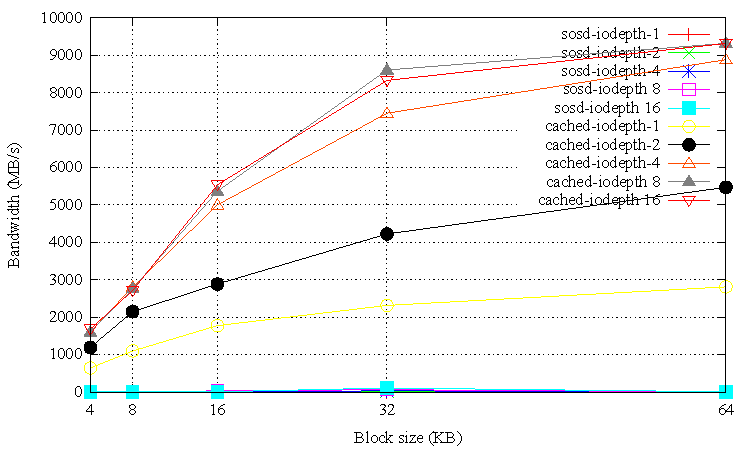
\includegraphics[]{diagrams/out.pdf}
	\caption{Cached vs. sosd}
	\label{fig:comp}
\end{figure}


Amazing results, right?

Let's see now the ugly truth...


